\chapter{算法与结果}
\label{cha:result}

\section{exRNA数据的收集与预处理}
\label{sec:first}

\subsection{exRNA数据收集}
我们收集整理了实验室自产的一套和两套发表的exRNA-seq数据,为了后续方便,我们称细胞外游离的RNA测序数据为cfRNA-seq,外泌体的RNA测序数据为exoRNA-seq. 同时我们用L(long)和S(small)区分长RNA和小RNA测序数据。一共四种主要的数据类型: S-cfRNA-seq, S-exoRNA-seq, L-cfRNA-seq, L-exoRNA-seq. 我们收集的数据的具体信息如下:S-exoRNA-seq 数据来自于 GEO 数据库中收录的 GSE71008 (\cite{yuan2016plasma}),包含健康供体(healthy donor, HD)的 50 个,结直肠癌100 个(colorectal cancer, CRC)样本,前列腺癌(prostate adenocarcinoma, PRAD)36 个。  S-cfRNA-seq ,我们整理了实验室内部产生的数据GSE123972 (\cite{tan2019noncoding}) 以及GSE113994(\cite{max2018human}),GSE53080(\cite{giraldez2018comprehensive}) 和 GSE94582(\cite{akat2014comparative});GSE123973 有可用的肝癌(hepatocellular carcinoma, HCC) 样本30例,其中包括早期肝癌(HCC stageA)16个,健康供体(HD)的 13 个样本。 GSE113994包含53健康供体,GSE53080包含17健康供体,GSE94582包含20健康供体。对于 L-exoRNA-seq 数据,我们收集exoRBase数据库(\cite{li2017exorbase})中的数据,其源于多个实验室的合作,包括肝癌样本14个,结肠癌样本12个,胰腺癌样本14个和健康供体32个。
数据总结如表~\ref{tab:exRNAsumtable}所示

\begin{table}[htb]
  \centering
  \begin{minipage}[t]{0.9\linewidth} % 如果想在表格中使用脚注,minipage是个不错的办法
  \caption[exRNA数据收集总结]{exRNA数据收集总结}%{模板文件。如果表格的标题很长,那么在表格索引中就会很不美}
  \label{tab:exRNAsumtable}
  %210pt in total
    \begin{tabularx}{\linewidth}{p{70pt}|p{80pt}|p{110pt}|p{70pt}}
      \toprule[1.5pt]
      {\heiti Data type} & {\heiti Sources}  & {\heiti Sample class} & {\heiti Sample size}\\\midrule[1pt]   
      S-exoRNA-seq & GSE71008 & \textbf{CRC}, PRAD, HD & 186\\
      S-cfRNA-seq & GSE123972 & \textbf{HCC}, HD & 43\\
      S-cfRNA-seq & GSE113994 & HD & 53\\
      S-cfRNA-seq & GSE53080 & HD & 17\\
      S-cfRNA-seq & GSE94582 & HD & 20\\
      L-exoRNA-seq & exoRBase & \textbf{HCC}, CRC, PRAD, HD & 20\\
      % (\cite{yuan2016plasma}) (\cite{tan2019noncoding}) (\cite{max2018human}) (\cite{giraldez2018comprehensive}) (\cite{akat2014comparative}) (\cite{li2017exorbase})
      \bottomrule[1.5pt]
    \end{tabularx}
  \end{minipage}
\end{table}

\paragraph{exRNA测序数据的处理}
针对exRNA数据微量性的特点,我们专门设计了小RNA测序数据的顺序比对方法,确定了其比对的先后顺序。完整的流程如图~\ref{fig:reads_processing}所示。包括数据清洗,质量控制,顺序比对(针对小RNA)或序列比对,以及构建表达矩阵,在构建表达矩阵时,针对小RNA测序中的长RNA(如Y RNA, lncRNA, snoRNA等),课题合作成员史斌斌还开发了专门的寻找其片段作为特征的方法。由于exRNA的微量性,不同样本间的各RNA比例变化很大,不论是确定比对顺序,还是做质量控制(quality control, QC)均需要精细的控制,我们使用丰富的可视化方法获得各类RNA的比例的统计结果,以及质量控制的结果总结等。接下来分别简要叙述长exRNA测序数据(L-exoRNA-seq)和小exRNA(s-exoRNA-seq, s-cfRNA-seq)测序数据的处理流程和结果。

\begin{figure}[H] % use float package if you want it here
    \centering
    \includegraphics[width = 0.8\textwidth]{reads_processing}
    \caption{reads处理流程图}
    \label{fig:reads_processing}
\end{figure}




\subsection{长exRNA测序数据的处理}

我们采用L-exoRNA-seq数据作为长exRNA数据,数据来自于exoRBase数据库(\cite{li2017exorbase}),测序类型为长RNA-seq双端(paired end)测序。我们首先用cutadapt工具实现对接头的剪切(trim adapter),因为是双端测序,我们要求只要其中任意一个read的质量分数低于30就会被滤除。我们首先将将reads比对到rRNA并且去除掉所有比对上的reads,这是因为显然rRNA不会被分泌到细胞外,不符合我们的要求。然后我们将reads比对到人类基因组(version: human genome 38),除此之外,我们还额外关注了circular RNA的信息,因此在比对到人类基因组之后,我们专门又将reads比对到circBase数据库。由于是双端测序,我们规定需要在互相配对的两条reads均比对成功的前提下才算作比对成功。长exRNA测序数据还有较为严重的因为qPCR扩增导致的duplication问题,因此我们还是用picard去除了duplicates,最后再使用featurecounts软件生成基因表达矩阵(基因计数矩阵)。

\paragraph{长RNA比对结果统计}
exSEEK可以自动统计出入图~\ref{fig:exorbase_basic} 所示的比对结果, (A) 表示不同RNA映射比例的饼图; (B) 表示不同RNA的长度分布的三维条形图;(C) 表示不同RNA的映射比例的箱线图 (D) 表示每个样本各种RNA映射比例的叠加条形图。
\begin{figure}[H] % use float package if you want it here
    \centering
    \includegraphics[width = 0.8\textwidth]{exorbase_basic}
    \caption{L-exoRNA-seq数据mapping基本情况统计。}
    \label{fig:exorbase_basic}
\end{figure}

可以看到长exRNA测序数据的结果中,绝大部分的reads比对到了mRNA和人类基因组上以及有较大比例没有比对上的reads。另外还有少量的circRNA,srpRNA,lncRNA等。我们在构建表达矩阵时并不使用miRNA和piRNA,因为exoRBase建库时使用的是双端150(PE150)测序,自动筛除掉了RNA长度较低的miRNA和piRNA。值得注意的是,虽然非编码RNA如circRNA,srpRNA,lncRNA等的绝对比例不高,但是后续分析可以发现发生差异表达的RNA中这些非编码RNA可能占有较高的比例,所以它们依然有作为生物标志物的潜力。



\subsection{小exRNA测序数据的处理}


我们采用S-exoRNA-seq和S-cfRNA-seq数据作为小exRNA数据,S-exoRNA-seq数据来自于 GEO 数据库中收录的 GSE71008 (\cite{yuan2016plasma}),S-cfRNA-seq来自于GSE123972(\cite{tan2019noncoding}) 以及GSE113994(\cite{max2018human}),GSE53080(\cite{giraldez2018comprehensive}) 和 GSE94582(\cite{akat2014comparative}),测序类型为小RNA-seq单端(single end)测序。


我们首先用cutadapt工具实现对接头的剪切(trim adapter),相比于双端测序,单端测序时只需要去除3’端的接头即可,我们同样要求reads的质量得分必须要于30分,且要求其长度必须在16个碱基长度到50个碱基长度之间。我们首选可选择地将reads比对到spikein序列上,然后是rRNA数据库以及载体数据库(UniVec)上(以去除被载体污染的reads)。接下来针对小RNA测序长度短,量小的问题,为了关注我们感兴趣的RNA,我们使用单独比对的方法,分别将reads按顺序比对到各个RNA注释数据库上,我们发现不同的比对顺序会造成各类RNA的比对比例产生较大的变化,因此我们在前期工作中探索了不同的比对顺序的影响,因为使用Bowtie2进行一次比对需要的时间很长,我们使用了专门设计的算法可以在一次比对后测定数十种不同的测序顺序各个RNA的比例,确定了我们关注的RNA如lncRNA,mRNA等的比例如何要求,最终确定了lncRNA、miRNA、mRNA、piRNA、snoRNA、snRNA、srpRNA、tRNA、 TUCP RNA、 Y RNA的比对顺序。对于无法比对到人类基因组的reads,我们将其比对到启动子,增强子,和重复区域(enhancer,promoter,repeats)等位置,最终将剩余的reads比对到circRNA上,对于依然无法比对的reads,我们将其命名为unmapped reads。

\paragraph{小RNA比对结果统计}
exSEEK可以自动统计出入图~\ref{fig:lulab_basic}所示的比对结果, (A) 表示不同RNA映射比例的饼图; (B) 表示不同RNA的长度分布的三维条形图;(C) 表示不同RNA的映射比例的箱线图 (D) 表示每个样本各种RNA映射比例的叠加条形图。
\begin{figure}[H] % use float package if you want it here
    \centering
    \includegraphics[width = 0.8\textwidth]{lulab_basic}
    \caption{S-cfRNA-seq数据mapping基本情况统计}
    \label{fig:lulab_basic}
\end{figure}

通过对比结果统计图可以看到,大多数的reads比对到了Y RNA,miRNA和rRNA上,snoRNA,enhancer和repeats也有一定比例的reads比对上。我们发现rNRA,miRNA和Y RNA不但比例较高,而且不同样本间的比例还有较大的差异,这可能是因为不同的样本存在一些批次效应(如RNA提取方法等的差异)。Y RNA的种类很少,只有四条,但是其丰度极大,有百分之四十左右的reads会比对到这四条RNA上。Y RNA是小的非编码RNA。它们是Ro60核糖核蛋白颗粒的组分,是系统性红斑狼疮患者的自身免疫抗体的靶标。它们也是通过与染色质和起始蛋白相互作用进行DNA复制所必需的。Y RNA在一些人类中过度表达,是细胞增殖所必需的,其分解产物也会参与到自身免疫和一些其他病理情况中(~\cite{hall2013rnas}),因此Y RNA也有潜在的区分癌症和正常样本的功能。值得注意的是circRNA在小RNA测序中的比例极低,不到万分之一,因此可能不能作为潜在的生物标志物使用,这和长exRNA测序中的结果不同,与长exRNA测序类似的是,虽然非编码RNA如lncRNA,snoRNA,tRNA等的绝对比例不高,但是后续分析可以发现发生差异表达的RNA中这些非编码RNA可能占有较高的比例,所以它们依然有作为生物标志物的潜力。




\section{表达矩阵的构建}
\label{sec:second}

完成了exRNA-seq数据的收集,预处理和比对后,我们进行了exRNA-seq数据的表达矩阵的构建。传统的表达矩阵构建只需要使用如featurecounts之类的软件工具即可。对于L-exoRNA-seq数据我们就是这么处理的。对于小exRNA-seq测序数据,我们采取了由课题合作成员史斌斌专门设计的结构域检测(domain calling)方法来发现结构域特征,并以结构域特征取代全长特征来构建表达矩阵。


\paragraph{小exRNA-seq测序数据的碎片化特征}
我们首先从exRNA-seq数据的比对部分获得图~\ref{fig:length_distribution},使用三维条状图和折线图展示了S-cfRNA-seq数据的各种类型RNA的长度分布。可以发现在S-exRNA-seq中,碎片化的情况非常严重,大多数的长RNA的reads长度也集中在20-30个碱基长度范围内。为此我们希望可以找到信噪比较高的reads覆盖区域更加集中的片段作为特征,以取代其全长特征。我们开发了一种专门针对 exRNA 数据的域检测算法,其总体设计思想与传统的根据read起始位置计算其覆盖值的peak calling软件Piranha类似,但是我们的方法可以做到更高灵的敏度以及找到更加准确的域位置。
\begin{figure}[h]
\centering%
\begin{subfigure}{0.4\textwidth}
\includegraphics[height=6cm]{3d_bar}
\caption{RNA长度分布的三维条形图展示}
\end{subfigure}%
\hspace{4em}%
\begin{subfigure}{0.4\textwidth}
\includegraphics[height=7cm]{length_distribution}
\caption{RNA长度分布的折线图图展示}
\end{subfigure}
\caption{RNA长度分布}
\label{fig:length_distribution}
\end{figure}


\paragraph{结构域可视化}
由于结构域检测算法主要由史斌斌同学完成,这里不再叙述其具体原理和过程,只展示相关的部分分析结果。为了展示exRNA-seq数据,尤其是小exRNA数据缺失存在明显的碎片化特征,我们比较了四套RNA-seq测序数据,两套来自小exRNA-seq数据,两套来自于组织RNA数据。我们以S-cfNRA-seq和S-exoRNA-seq的每个峰的中点作为原点坐标进行覆盖度的可视化,如图~\ref{fig:domain_size}所示,可以看到对于exRNA数据,在峰的周围有非常显著的reads覆盖度的凸起,高于周围的区域,而对于组织RNA数据则没有明显的峰存在。我们还对exRNA的结构域长度统计,发现大多数结构域片段的长度集中在30个碱基长度左右,很少超过100个碱基长度,这进一步佐证了exRNA测序数据的大多数reads都以碎片化形式存在,而不是全长形式。


\begin{figure}[h]
  \centering%
  \begin{subfigure}{0.4\textwidth}
    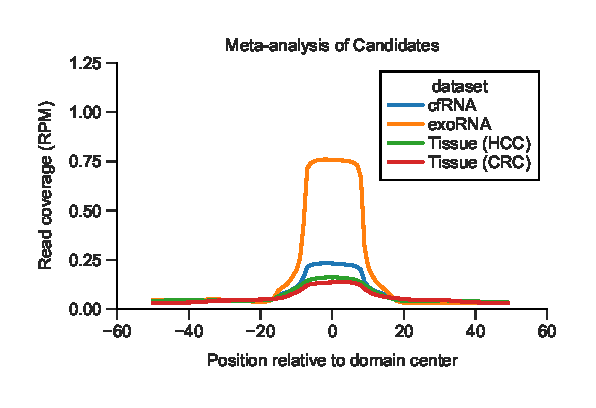
\includegraphics[height=5cm]{aggregation_plot}
    \caption{结构域分布}
  \end{subfigure}%
  \hspace{4em}%
  \begin{subfigure}{0.4\textwidth}
    \includegraphics[height=5cm]{domain_size}
    \caption{结构域大小分布}
  \end{subfigure}
  \caption{不同exRNA和组织数据结构域分布和大小分布}
  \label{fig:domain_size}
\end{figure}


\paragraph{表达矩阵的数据统计}

最终对于小exRNA-seq测序数据,我们构建了由长RNA的结构域特征加miRNA全长特征合并的表达矩阵,对于长exRNA-seq数据,我们直接适用featurecounts构建全长特征,作为下一步表达矩阵处理的输入。对于我们专门使用结构域检测算法特殊处理的小exRNA测序数据的表达矩阵, 我们还做了如下的可视化分析。如图~\ref{fig:div_abu}所示,对于S-cfRNA-seq数据,我们发现miRNA,Y RNA和lncRNA占据了较高的丰度,但是由于使用了结构域检测算法,一些非编码RNA如snoRNA、tRNA、tucpRNA、snRNA和srpRNA均可以有较多的种类被检测到,显示出结构域检测算法可以帮助提供非编码RNA在表达矩阵中的多样性和种类数量。对于S-exoRNA-seq数据同样也可以观察到这样的特征,甚至更加明显,其中几种丰度非常微量的RNA如snRNA、lncRNA、mRNA、tucpRNA、srpRNA和snoRNA经过结构域检测算法,可以得到非常多样的特征。

\begin{figure}[h]
  \centering%
  \begin{subfigure}{0.4\textwidth}
    \includegraphics[height=3.5cm]{diversity_abundance_cfRNA}
    \caption{S-cfRNA-seq结构域和miRNA特征的丰度与多样性}
  \end{subfigure}%
  \hspace{4em}%
  \begin{subfigure}{0.4\textwidth}
    \includegraphics[height=3.5cm]{diversity_abundance_scirep}
    \caption{S-exoRNA-seq结构域和miRNA特征的丰度与多样性}
  \end{subfigure}
  \caption{小exRNA-seq结构域和miRNA特征的丰度与多样性}
  \label{fig:div_abu}
\end{figure}

进一步地为了检测这些特征是否对于区分癌症和正常样本有用,我们绘制了如图~\ref{fig:diff_pie}所示的差异表达分析中各类RNA所占比例的饼图。我们发现虽然miRNA在exRNA-seq数据中的丰度很大,但是其在S-cfRNA-seq和S-exoRNA-seq的差异表达基因中所占的比例只有20\%左右,这进一步说明了其他丰度较低的RNA其实具有很高的多样性,而且有潜力作为区分癌症和正常样本的生物标志物,作为过去被广泛研究的miRNA癌症生物标志物的补充。

\begin{figure}[h]
  \centering%
  \begin{subfigure}{0.4\textwidth}
    \includegraphics[height=4cm]{piecharts_cfRNA}
    \caption{S-cfRNA-seq差异表达RNA比例}
  \end{subfigure}%
  \hspace{4em}%
  \begin{subfigure}{0.4\textwidth}
    \includegraphics[height=4cm]{piecharts_scirep}
    \caption{S-exoRNA-seq差异表达RNA比例}
  \end{subfigure}
  \caption{小exRNA-seq差异表达RNA比例}
  \label{fig:diff_pie}
\end{figure}

\section{表达矩阵的处理}
\label{sec:third}

在矩阵处理部分,我们进行了如图~\ref{fig:mx_process_pipe}的顺序处理过程,包括过滤与归责,样本库大小归一化(测序深度归一化),去除批次效应等步骤。我们将不同的处理方法进行组合,并对每个步骤进行了单独的和综合的评估,使用了非监督聚类准确性(unsupervised clustering accuracy, UCA)
和m-K最近邻 (m-K-nearest neighbor, mKNN)两个指标综合选取最佳的矩阵处理方法组合。本部分的矩阵处理代码由R语言实现,评估指标由python实现。


\begin{figure}[H] % use float package if you want it here
    \centering
    \includegraphics[width = 0.7\textwidth]{matrix_processing}
    \caption{表达矩阵处理流程图}
    \label{fig:mx_process_pipe}
\end{figure}

\subsection{过滤与归责处理}
我们首先是用了过滤和归责处理(imputation)的方法对表达矩阵进行处理。因为exRNA数据的稀疏化特征,是用过滤和归责是很常规的想法。


由于exRNA中有大量的缺失值,因此过滤掉一些整体表达值很低的基因是常见的做法。exSEEK可以自己设置过滤的条件,比如对于原始基因计数矩阵,或者counts per millio(CPM), reads per kb per million reads(PRKM)进行过滤,默认设置为过滤掉基因计数矩阵中表达值小于5的样本超过50\%的那些基因。

\paragraph{归责处理}
归责处理即对数据中的缺失值进行推断和插补,我们使用scImpute(\cite{li2018accurate})进行归责处理,scImpute的思想如图~\ref{fig:scimpute}:

\begin{figure}[H] % use float package if you want it here
    \centering
    \includegraphics[width = 0.7\textwidth]{scimpute}
    \caption{scImpute原理}
    \label{fig:scimpute}
\end{figure}

\begin{itemize}
\item 首先,使用一个混合模型(mixture model)学习每个细胞中每个基因存在缺失的概率。
\item 接着,插补很大概率为缺失值的基因。首先将基因分为较大程度受到缺失影响的集合$A_j$和没有受到缺失值较大影响的集合$B_j$,然后根据$B_j$的基因首先做主成分分析,找到解释性较大的几个主成分,利用这几个主成分的矩阵对样本进行聚类。
\item 根据聚类结果,可以将样本分为有较高可能有缺失值和较高可能性表达值正常测定的两类,对表达值正常的样本进行线性回归,并将权重用于较高可能缺失的样本上,就完成了对缺失值的插补。
\end{itemize}

\subsection{样本库大小归一化}

对样本库大小(library size)进行归一化的原因在于实验中不同样本的计数总数会受到实验时的诸多因素影响(如PCR扩增倍数,测序深度等),造成样本间同种基因的计数有差异。对于RNA$-$seq数据,我们通常认为这种影响因素对于每个基因是等比例的,然而对于量较少的exRNA-seq以及单细胞测序,也有理论认为对于样本内部的不同基因,也应该使用不同的归一化因子,单细胞测序的归一化方法之一SCnorm(\cite{bacher2017scnorm})即采取这种策略。基本的样本库归一化方法是将每个样本的所有基因的原始reads各乘以一个归一化因子,保证各个样本的样本库大小在归一化后一致。我们选择了多种归一化方法:CPM,  CPM\_top, TMM, RLE, UQ, SCnorm.

\paragraph{样本库大小归一化方法原理简介}\mbox{}\\

CPM(counts per million)通过对样本的所有reads求和得到样本库大小,每个基因的reads数除以该样本总reads数再乘以$10^6$即为归一化后该基因的表达值。

我们对CPM做了一些修改,CPM\_top算法对于top20表达量的基因和其余基因分别使用不同的归一化因子进行归一化,这是考虑到exRNA-seq数据中表达量前20的基因可以占据reads总数的50\%以上,分别归一化可以避免表达量极大的基因对其余基因的分布的影响,这和SCnorm的想法比较类似。

UQ(upper quartile)(\cite{love2014moderated})对 CPM 进行一些修改,与CPM\_top类似。UQ用在至少一个样本中表达的基因 reads 数的上四分位数(75\%分位数)来作为样本库大小进行归一化。这样可以避免一些表达量特别大的基因对剩余基因的影响,一定程度上避免差异表达分析的假阳性。

TMM(trimmed mean of M-values)(\cite{diaz2006gene})略微复杂。对每个样本,把其他样本作为比较样本,计算一个系数。去掉样本中表达值的很大的极端值,每个比较样本与本样本分别计算对数比例,加权求和得到每个样本各自的归一化因子。可以看出如果基因没有差异表达,那么系数应该接近1,事实上大多数基因确实是没有差异表达的,因此TMM可以用于校正技术因素导致的系数偏离1的情况。

RLE(relative log expression)(\cite{anders2012detecting})对每个基因,首先计算每个基因的样本间几何平均,对每个样本,计算每个基因的reads 数与对应的几何平均的比值,取每个样本所有比值的中位数作为RLE系数。RLE也假设了大多数基因是没有差异表达的,因此RLE也接近1,偏离1的RLE系数可以被用来做样本库大小的归一化。


RLE 图可以用于显示样本库大小归一化前后的变化。RLE图和RLE归一化思想是一样的,对于每个样本,如果大多数基因没有差异表达,上述的RLE系数,即每个样本的reads数与基因跨样本几何平均的比值的中位数应该接近0。图~\ref{fig:rle}展示了使用RLE作为归一化方法的效果:从中可以看到在归一化之前,数据GSE123972的RLE系数明显大于0,不同的数据集的测序深度很不一样,经过计算可以得到所有数据的RLE系数相对于0的偏离为4.25,归一化之后不同数据的异质性明显减小,而且variance分数明显降低为0.45,体现出RLE具有较好的归一化效果。





\begin{figure}[H] % use float package if you want it here
    \centering
    \includegraphics[width = 0.8\textwidth]{RLE}
    \caption{样本库大小归一化效果}
    \label{fig:rle}
\end{figure}

\subsection{去除批次效应}

批次效应指人为引入的技术差异(technical variance)使得样本不按照真正的类别信息聚类,而是向人为造成的批次偏移,如不同的实验日期,不同的建库大小,胶选择长度等都会造成批次效应。我们依据数据来源文献中所指明的批次效应,采用了RUV(\cite{risso2014normalization}),ComBat(\cite{chen2011removing}),Limma(\cite{ritchie2015limma})等方法进行批次效应的去除。并且使用m-K最近邻 (m-K-nearest neighbor, mKNN)指标来衡量批次效应的去除效果。



limma使用线性回归对每个样本的每个基因的计数值进行校正,并不要求计数必须为整数值,即可以输入经过归一化的数值。事实上Limma要求输入的数据分布更加紧凑,所以可以取对数作为输入。Limma假设基因的表达值符合固定因素和随机因素的加性效应,固定效应包括批次效应和其他技术因素引入的差异。因此Limma可以建立一个线性模型,以批次效应的信息作为自变量,以基因表达值作为因变量进行回归,再用基因表达值减去固定效应值,得到校正表达值。所以Limma要求一定要有批次信息作为输入。


ComBat生成实现了比Limma更加适用于小数据的批次效应去除方法。其原理在于线性回归的参数估计可能会受到极端值影响。ComBat使用一种经验贝叶斯的方法,对批次效应值实现层次的估计,即为了估计批次效应值服从的先验分布,而该先验分布的参数也服从另一个分布,由一组超参数控制,经验贝叶斯使用频率学派的估计方法估计超参数,再用贝叶斯方法估计先验分布,对于小样本数据的噪音具有更强的鲁棒性。

RUV适用于批次效应信息不可获得或者不希望按照已有的批次信息进行完全去除的情况(如批次信息与样本类别信息重合过大)。RUV可以先进行差异表达分析,去除差异表达的因素,即生物学差异后,再进行因子分析来寻找潜在的批次效应,用户可以设置一个k值,作为RUV进行线性回归时的隐变量个数控制,越大的k代表RUV的潜在批次越复杂。


对于批次信息存在且与样本类别信息差异不大的情况,可以使用以上三种批次效应去除方法,以及不使用批次效应去除方法作为对比,否则可以使用RUV对不输入批次效应信息的数据进行批次效应去除。

批次效应的去除可以通过降维可视化的方式鉴别,我们将在图~\ref{fig:matrix_processing_metric}
展示,直观上来看,同一批次的样本越分散,也就是不同批次的样本混合越均匀,则批次效应的影响越小,去除批次效应的效果越好。另一种展示方法通过方差分解(variance decomposition analysis)。将表达值作为因变量,可以将各种因素分别作为自变量回归,如样本信息,批次信息,样本库大小等。对于每个基因作为因变量,都可以计算出不同的自变量解释的方差与总方差的比值,对于每一种自变量,都可以画出来其对每个基因的方差贡献比的分布曲线。图~\ref{fig:batch_correction}所示,以批次效应信息作为自变量时,去除批次效应后,方差贡献分布曲线明显左移(蓝线到红线),说明批次效应对基因表达值的影响变小。而以样本类别信息作为自变量时,虽然方差贡献分布曲线也有左移,但是左移相对于批次效应的曲线明显较小,可以认为我们在去除批次效应的同时较好地保留了不同类别样本的差异性,即生物学效应带来的组间差异。

\begin{figure}[H] % use float package if you want it here
    \centering
    \includegraphics[width = 0.65\textwidth]{batch_correction}
    \caption{去除批次效应效果}
    \label{fig:batch_correction}
\end{figure}

\subsection{评估表达矩阵处理效果}



非监督聚类准确性(unsupervised clustering accuracy, UCA)(\cite{lopez2018deep}),由一篇单细胞领域研究中首次适用,用于衡量聚类的效果,作为PCA和t-SNE等降维可视化分析的量化评估,可以使我们预先判断当前处理效果下数据的大致分类效果。
UCA首先只用K-means(\cite{jain1988algorithms})或者KNN(\cite{cover1967nearest})作为聚类的方法,由于是非监督聚类,还需要使用线性分配的算法如匈牙利算法(\cite{linearassign})将聚类标签与真实标签进行匹配。此时该问题可以看做一个有标签的分类问题,计算出分类的准确率即为非监督聚类准确性。
对于多种不同的聚类度量指标,我们发现UCA和有监督的分类度量指标AUC具有最强的相关性,因此采用非监督聚类准确性指标作为矩阵处理效果的度量之一。

为了更好地衡量批次效应的严重性以及批次效应去除效果,我们参考了过去的指标如对齐分数(alignment score)(\cite{butler2018integrating}),和kBET(\cite{buttner2017assessment})两个研究。对齐分数虽然计算简单,但是只适用于二分类标签,kBET使用时会遇到受到随机效应影响而导致极端值附近的结果不够稳定的情况。
为此我们提出了m-K最近邻 (m-K-nearest neighbor, mKNN)指标, 公式如式~(\ref{eq:mknn})所示,其中 $\bar x_b, k, N_b, N, B$ 分别表示:批次为b的样本周围同类批次的样本平均个数,自主定义的最近邻取样数,批次为b的样本总数,所有样本的总数以及批次的种类数。利用mKNN指标,我们可以逐批次逐样本地衡量其批次效应的严重性,
批次效应越严重,则分子中的$\bar x_b$越大,相应的整个指标越大。为了更好地表示“去除批次效应的效果”,我们使用1-mKNN作为去除批次效应效果的指标。
\begin{equation}
\label{eq:mknn}
\frac { 1 } { B } \sum _ { b = 1 } ^ { B } \frac { \overline { x } _ { b } - k N _ { b } / ( N - 1 ) } { \min \left( k , N _ { b } \right) - k N _ { b } / ( N - 1 ) }
\end{equation}

UCA和mKNN指标均为$0\sim 1$,数值越大代表聚类效果越好以及批次效应的影响越小。因此我们统一地考虑两个指标,将矩阵处理方法的组合(即测序深度归一化以及去除批次效应方法的组合)加以统一的评估。图~\ref{fig:matrix_processing_metric}中每一个点表示一种矩阵
处理方法的组合。越靠近右上角的指标代表矩阵处理效果越好。如图所示,我们可以选择RLE作为测序深度归一化加上Limma作为去除批次效应的方法组合。对于该方法组合,我们还是用了PCA对矩阵处理前后的数据进行了可视化,PCA可以用于降维,选择方差贡献最大的两个主成分表示到二维平面上,点的颜色表示批次,性状表示类别信息。
不管是视觉上观察可以看到不同批次的点更好的混在了一起,还是从两个指标的变化($\text{UCA}:0.519 \rightarrow 0.692; \text{mKNN}:0.055 \rightarrow 0.792$)上,均可以得出矩阵处理方法较好地完成了测序深度归一化以及批次效应去除的任务的结论。

\begin{figure}[H] % use float package if you want it here
    \centering
    \includegraphics[width = 0.8\textwidth]{matrix_processing_metric}
    \caption{综合使用UCA和mKNN评估矩阵处理效果}
    \label{fig:matrix_processing_metric}
\end{figure}

\section{特征选择和模型评估}
\label{sec:fourth}
由矩阵处理流程处理好的表达矩阵消除了部分技术性差异(technical variance)导致的样本库大小不一致和批次效应问题。
我们可以对处理过的表达矩阵应用一些统计学习模型,设计一套特征选择流程,选取对于癌症和正常样本分类效果好的,稳定的,具有生物学意义的特征,作为癌症检测的潜在的生物标志物。

\subsection{差异表达分析}
差异表达分析可以使用统计模型逐基因地寻找在癌症和正常人之间差异表达的特征。因为也可以作为
特征选择的基本方法之一。


% 讨论deseq的基本原理,注意表达要修改
我们使用DESeq2包进行差异表达分析,值得注意的是DESeq2专门要求输入的矩阵必须是基因计数矩阵,也就是未经标准化和归一化的表达矩阵(un-normalized counts)(\cite{love2014moderated}). 因为这样的矩阵具有最多的信息和准确性,DESeq2在内部会自动完成归一化的工作。

DESeq2为了比较两组样本之间的计数差异建立了一个模型。该模型包含以下参数:(1)归一化参数,至少可以归一化库大小的差异; (2)方差参数,也被成为分散系数(dispersion); (3)表示组间差异的参数。DESeq2使用与原始DESeq相同的方法拟合(1)。拟合(2)分两步:首先找到使似然(likelihood)最大的参数值,即完成最大似然估计。查找所有的基因表达值,并将这些值向中间值移动,移动的量由贝叶斯模型给定:如果基因的信息较低,则值更多地移动到中间,如果基因的信息很大,则值移动很少。使用与(2)中使用的相同的技术拟合(3)。 (3)的值是最终需要得到的输出,找到一组组间差异高于某个数值的基因集合。这个阈值一般由错误发现率(False Discovery Rate, FDR)规定,一般取从小到大排最小的十个FDR基因作为差异表达基因。

对于差异表达基因的选取,这里我们使用一个改进的指标以替代FDR,该指标如公式~\ref{equ:demetric}所示,可以综合性考虑FDR和fold change,更加完善。

\begin{equation}\label{equ:demetric}
  \pi = \Vert \log _ { 2 } F C \Vert \cdot \left( - \log _ { 10 } \mathrm { FDR } \right)
\end{equation}


%compare counts between two groups. We build a model for the observed counts. This model has some parameters: (1) a normalization parameter, for differences in library size at least, or it can be extended by other software; (2) a variance parameter, called dispersion; (3) parameters representing the group differences. Fit (1) using the same method from the original DESeq. Fit (2) in two steps: first find the value of the parameter that makes the  likelihood largest, which iscalled maximum likelihood estimation. Look at all the values from all of the genes and move these values towards a middle value. Bayes theorem guides the amount of movement for each gene: if the information for the gene is low, the value is moved more to the middle, if the information for the gene is high, the value is moved very little. Fit (3) using the same technique as used for (2). The values for (3) are a useful final product, as are sets of genes where the group differences are likely to be above a threshold (zero or otherwise). These sets are defined by their false discovery rate.

%TODO 展示基本的DE结果并简单讨论
使用DESeq2对原始的基因计数矩阵进行分析,可以得到如图~\ref{fig:lulab_de}和图~\ref{fig:scirep_de}的结果。


对于~\ref{fig:lulab_de},我们使用S-cfRNA-seq数据,癌症类型分别为肝癌和早期肝癌。将其分别与正常样本比较,可以分别找出可以区分正常样本与肝癌以及正常样本与早期肝癌的差异基因。(A) 表示每个基因的对数fold change和对数调整后p值的火山图,图中红色的点为差异表达的基因,越靠近右上和左上的基因其差异表达越明显; (B) 前十个差异表达基因的fold change, 表达值以及对数调整后p值; (C) 挑选出的差异表达基因的热图以显示其对于癌症和正常样本的分类效果。
\begin{figure}[H] % use float package if you want it here
    \centering
    \includegraphics[width = 0.8\textwidth]{lulab_de}
    \caption{S-cfRNA-seq数据的差异表达分析}
    \label{fig:lulab_de}
\end{figure}

对于图~\ref{fig:scirep_de},我们使用S-exoRNA-seq数据,癌症类型分别为结肠癌和早期结肠癌。图的具体信息与图~\ref{fig:lulab_de}表示的类似。
\begin{figure}[H] % use float package if you want it here
    \centering
    \includegraphics[width = 0.8\textwidth]{scirep_de}
    \caption{S-exoRNA-seq数据的差异表达分析}
    \label{fig:scirep_de}
\end{figure}

差异表达分析的模型一般会独立考虑每个特征(即基因)的贡献,并不能结合性地讨论特征对分类的共同贡献,因此有局限性。接下来我们将会使用一些经典的机器学习模型来更好地组合不同的特征,以选出一组生物学上更有解释性和代表性的基因作为可能的生物标志物。同时考虑到模型必须具有的泛化能力以及稳定性,我们还会针对性地设计一个特征选择的框架来更好的挑选特征。

\subsection{特征选择策略与机器学习模型}




%~\ref{fig:fs_frame}
%\begin{figure}[H] % use float package if you want it here
%    \centering
%    \includegraphics[width = 0.6\textwidth]{fs_frame}
%    \caption{特征选择框架}
 %   \label{fig:fs_frame}
%\end{figure}

特征选择方法通常使用一些经典的机器学习模型用于将不同的样本类别进行区分(如区分肝癌和正常样本)。通过优化机器学习模型使其更好地区分组间差异,获得更好的分类效果的同时,我们往往可以分析模型的参数,得到每个特征对分类效果的贡献,即权重。通过寻找权重大的特征,我们可以找到对模型分类贡献最大的基因,也就是我们希望寻找的潜在的生物标志物。与差异表达的逐个基因判断其贡献相比,机器学习模型的建模假设可以更复杂,可以综合考虑基因间的关联性,甚至建立非线性的模型刻画这种关系,因此对数据有更好的建模效果,往往也可以获得更好的分类效果。然而由于模型的参数更复杂,对于数据的表示能力更强,往往也会带来严重的过拟合问题(~\cite{domingos2012few})。对于exRNA-seq数据的标志物发掘,我们还需要考虑实际的生物学意义,寻找稳定的,解释性强的特征,这要求我们更好地固定机器学习模型,减少特征选择算法的随机性。针对这些考虑,我们设计了如下的特征选择算法:

\paragraph{特征选择算法}

\begin{algorithm}
  \caption{稳健的特征选择算法}\label{alg:fs_algorithm}
  \begin{algorithmic}[1]
  \STATE Scale each feature independently using robust normalization;
  \FOR{feature\_num $k \in [1,10]$}
  \STATE Random select 90\% samples for 50 times;
  \STATE Run a classifier (Random Forest, Logistic Regression or Linear SVM) to select features based on feature importance. 
    \FOR{each classifier $\in$ [Random Forest, Logistic Regression or Linear SVM]}
    \STATE Optimize classifier's hyper-parameters by 5-fold cross-validation;
    \ENDFOR
  \STATE Select top k features that are recurrently selected across resampling runs;
  \STATE Calculate AUC mean;
  \ENDFOR
  \STATE Rank processing method by AUC, select the best $k$;
  %\STATE Select union of features in different feature\_num setting. Refit by selecting $i \in [1,10]$ features and calculate feature importance.
  \end{algorithmic}
  \end{algorithm}

  
特征选择的详细算法可以由Algorithm ~\ref{alg:fs_algorithm}得到。首先,不同于DESeq2要求输入未经归一化的表达值,特征选择算法可以输入经过了归一化和去除批次效应的表达值。我们之前只对样本进行了库大小的归一化,一般而言还要对特征进行逐个标准化。公式~\ref{eq:robustnorm}表示robust normalization的具体做法,对于每个特征,通过减去其中位数,除以四分间距(IQR: Interquartile Range),即可得到标准化后的表达值,使用四分间距作为分母而不是标准差,可以有效避免极端值对标准化的影响,具有更强的鲁棒性。
\begin{equation}\label{eq:robustnorm}
  \text { robust\_scale } \left( x _ { i j } ^ { \prime } \right) = \frac { x _ { i j } - \operatorname { median } _ { k } x _ { i k } } { Q _ { 0.75 } \left( \mathbf { x } _ { i } \right) - Q _ { 0.25 } \left( \mathbf { x } _ { i } \right) }
\end{equation}


接着,由于我们对于最终选择的特征的数量尚未确定,我们首先需要测试挑选的特征的数量,即$k \in [1,10], 20, 30, 40, 50$. 为了挑选出稳健的特征,我们对每个$k$都要进行50轮的测试,挑选在测试中反复出现的特征。由于样本量本身较小,我们没有采用交叉验证(cross validation)的方法,而是直接将全部数据集在每次测试中划分为90\%的训练集和10\%的测试集。在每轮测试中,训练集和测试集的样本都有随机不放回抽样决定,保证训练集中的各类样本的比例与总体类似。我们会使用多种机器学习模型,如逻辑斯谛回归(\cite{kleinbaum2002logistic}),支持向量机(\cite{scholkopf2001learning}),随机森林(\cite{liaw2002classification})等。在每轮测试,我们都会进行五折的交叉验证(5-fold cross validation)以优化机器学习模型内部的超参数,这些超参数不能由模型自己优化得到,而必须通过人为的选择,比较不同超参数设定时的结果来得到,比如逻辑斯谛回归中的C来控制正则化(regularization)的大小的倒数,C越小代表越强的正则化,随机森林中有树的个数和最大深度作为超参数。最终我们选取50轮测试中重复出现的特征,重新使用机器学习模型选择权重贡献最大的$k$个特征作为最终选择的特征。在50轮的测试中我们可以计算出50轮的平均分类准确度指标:AUC的平均值。之后我们可以选择最佳的$k$,在尽可能保证较高的AUC的情况下减少$k$的值。

%feature selection算法





\paragraph{机器学习模型}
在特征选择框架中我们可以选择多种机器学习模型,包括逻辑斯谛回归,支持向量机,随机森林等。
以逻辑斯谛回归为例,对于二分类问题,逻辑斯谛回归的决策模型如公式~\ref{equ:logistic}所示,其中$x$为表达矩阵,$\beta$为逻辑斯谛回归中线性模型的权重向量,$\beta_0$为偏置项。公式~\ref{equ:logistic}表示输入为$x$时模型判断样本标签为1的概率。若设患癌症样本的标签为1,则代表该样本为癌症患者的概率。
\begin{equation}\label{equ:logistic}
    P ( Y = 1 | X = x ) = \frac { \exp \left( \beta _ { 0 } + x ^ { T } \beta \right) } { 1 + \exp \left( \beta _ { 0 } + x ^ { T } \beta \right) }
\end{equation}

类似地可以得到多分类的逻辑斯谛回归如公式~\ref{equ:multilogistic}。当逻辑斯蒂回归模型获得数据输入,进行了训练后,为了最大化分类正确的概率,模型会内部优化出$\beta_0, \beta$的最优值,通过寻找$| \beta |$最大的那些值,即可找到我们希望寻找的,对于分类最有效的特征。

 
\begin{subequations}\label{equ:multilogistic}
\begin{flalign}
    & P ( Y = k | X = x ) = \frac { \exp \left( \beta _ { k , 0 } + x ^ { T } \beta _ { k } \right) } { 1 + \sum _ { l = 1 } ^ { K - 1 } \exp \left( \beta _ { l , 0 } + x ^ { T } \beta _ { l } \right) } , \text { for } k = 1 , \ldots , K - 1\\ 
    & P ( Y = K | X = x ) = \frac { 1 } { 1 + \sum _ { l = 1 } ^ { K - 1 } \exp \left( \beta _ { l , 0 } + x ^ { T } \beta _ { l } \right) } , \text { for } k = K
\end{flalign}
\end{subequations}



\subsection{特征选择的分类效果和稳健性评估}

\paragraph{分类效果衡量指标AUC}
为了衡量模型的分类效果,我们使用了曲线下面积(Area Under Curve, AUC)来衡量其分类效果,AUC是一个0-1之间的数字,对于二分类模型,完全随机分类的AUC为0.5,完全区分两类样本时的AUC为1,AUC越大代表分类效果越好。

对于样本的预测,我们使用医学和生物领域常用的混淆矩阵来计算其相应的指标,并进一步获得AUC的值。首先我们使用如表~\ref{tab:confusion_mx}所示的混淆矩阵来计算真阳性(True Positive Rate, TPR)和伪阳性(False Positive Rate, FPR),其中真阳性率也被称为灵敏度(Sensitivity),伪阳性率与特异度(Specificity)的关系为$1 - \text{FPR} = \text{Specificity}$。由于机器学习模型可以预测出每个样本分别属于两类别(癌症和正常人)的概率,因此对每个样本的二分类预测概率,选取一系列的截断值(cutoff),就可以用于构建多个混淆矩阵,并计算出每一个混淆矩阵的TPR和FPR值。将同一模型每个阈值的 (FPR, TPR) 座标都画在ROC空间里,就可以生成特定模型的ROC曲线(~\cite{roc_curve})。ROC曲线在完全随机预测时就是$y=x, x \in [0,1]$的直线,ROC曲线下围的面积就是AUC,AUC越接近1代表分类效果越好。

\begin{table}[htbp]
  \centering
  \caption{混淆矩阵}
  \label{tab:confusion_mx}
  \begin{minipage}[t]{0.9\textwidth} 
\begin{tabularx}{\linewidth}{p{45pt}|p{100pt}|p{100pt}|p{90pt}}
\hline
\diagbox[width=58pt]{\textbf{Predict}}{\textbf{True}} & \textbf{Positive}  &   \textbf{Negative} & \textbf{Metric}\\ \hline
\textbf{Positive} & True Positive (TP) & False Positive (FP) & $\textbf{PPV} =\frac{TP}{TP+FP}$ \\ \hline
 \textbf{Negative} &  False Negative (FN) &  True Negative (TN) &  $\textbf{NPV} =\frac{TN}{TN+FN}$ \\  \hline
 \textbf{Metric} & $\textbf{Sensiticity} = \frac{TP}{TP+FN}$ & $\textbf{Specificity} = \frac{TN}{TN+FP}$  & \\  \hline
\end{tabularx}
\end{minipage}
\end{table}


\paragraph{特征稳定性衡量指标KI}
挑选出重复性强的稳定的特征在液体活检领域非常重要,在不同测试轮数中重复出现的特征不仅对分类很重要,而且可能具有泛化能力强的特点。为了衡量挑选的特征的稳定性,我们使用了Kuncheva index (KI)来衡量特征的稳定性,
其公式如式~(\ref{eq:ki}),其中 $f_i, f_j$ 为两次挑选的特征,$d, N$ 分别为一次挑选的特征数和总特征数量。
\begin{equation}\label{eq:ki}
\mathrm { KI } \left( f _ { i } , f _ { j } \right) = \frac { \left| f _ { i } \cap f _ { j } \right| N - d ^ { 2 } }{ d N - d ^ { 2 } } = \frac { \left| f _ { i } \cap f _ { j } \right| - d ^ { 2 } / N } { d - d ^ { 2 } / N }
\end{equation}

若做K次采样,均采取不放回的策略时,可以获得平均KI的公式如式~(\ref{eq:aki}),即AKI。

\begin{equation}\label{eq:aki}
\mathrm { AKI } = \frac { 2 } { M ( M - 1 ) } \sum _ { i = 1 } ^ { M } \sum _ { j = 1 } ^ { M } \mathrm { KI } \left( f _ { i } , f _ { j } \right)
\end{equation}

KI和AKI同样为0-1之间的值,其值越接近1则代表特征越稳定,AKI为1时代表多轮测试中挑选出的权重最大的特征完全一致,这是最理想的情况。


\subsection{模型分类效果比较总结}

为了更好的比较exSEEK挑选出的生物标志物和已知的一些经典的生物标志物,我们总结了各类生物标志物和exSEEK挑选出的特征的AUC用以比较,我们首先注意到如
图~\ref{fig:compare_feature_num}所示,在挑选10个以下的特征时,特征的数量变化并不会造成AUC的剧烈变动,挑选6-7个甚至更少的特征也可以取得很好的分类效果。
\begin{figure}[H] % use float package if you want it here
    \centering
    \includegraphics[width = 0.8\textwidth]{compare_feature_num}
    \caption{挑选不同数量feature时AUC的变化}
    \label{fig:compare_feature_num}
\end{figure}


表~\ref{fig:table_auc}分别总结了结肠癌和肝癌的不同已知生物标志物和exSEEK挑出的生物标志物的AUC总结。
其中第一行的CRC/HD, CRC\_S1/HD, HCC/HD, HCC\_S1/HD分别代表结肠癌和正常人,结肠癌早期和正常人,肝癌和正常人,肝癌早期和正常人的比较。
第二行的Mean,std\_dev和rounds分别代表测试的AUC的均值,标准差和测试轮数。第一列的methods表示该marker是使用原始文献的参数还是使用exSEEK优化得到的参数进行分类。
第二列代表选择的生物标志物,标志物名称的括号中的数字表示其使用的基因的数量。每个表格的前两个标志物(miR-20, miRNA6; miR-21, miRNA7)为已知的生物标志物,使用其原始文献中的参数进行测试。
miRNA6, miRNA7还通过exSEEK进行了重新优化,其结果得到了显著提升。ncRNA和miRNA\_only分别代表exSEEK发现的非编码RNA生物标志物组合以及仅包含miRNA的生物标志物组合。


\begin{figure}[h]
  \centering%
  \begin{subfigure}{0.6\textwidth}
    \includegraphics[height=3cm]{hcc_bio_table}
    \caption{结肠癌各生物标志物AUC指标统计表}
  \end{subfigure}%
  \hspace{4em}%
  \begin{subfigure}{0.6\textwidth}
    \includegraphics[height=3cm]{crc_bio_table}
    \caption{肝癌各生物标志物AUC指标统计表}
  \end{subfigure}
  \caption{特征选择方法总结}
  \label{fig:table_auc}
\end{figure}

图~\ref{fig:hcc_crc_auc_sum}汇总了表~\ref{fig:table_auc}的具体结果,以条形图加以展示。使用exSEEK,我们比较了已知的生物标志物和由exSEEK优化或挑选出的生物标志物的分类结果。可以看到由exSEEK挑选的ncRNA取得了最好的分类效果,而经过exSEEK优化的已知的生物标志物(第三栏)比该标志物原始参数设定下(第二栏)的分类结果获得了一定的提升。
\begin{figure}[h]
  \centering%
  \begin{subfigure}{0.4\textwidth}
    \includegraphics[height=5cm]{hcc_auc_sum_revise_fig4b_5_commer}
    \caption{肝癌各生物标志物AUC总结}
  \end{subfigure}%
  \hspace{4em}%
  \begin{subfigure}{0.4\textwidth}
    \includegraphics[height=5cm]{crc_auc_sum_revise_fig4b_5_commer}
    \caption{结肠癌各生物标志物AUC总结}
  \end{subfigure}
  \caption{肝癌和结肠癌AUC总结}
  \label{fig:hcc_crc_auc_sum}
\end{figure}



\paragraph{各类癌症在各个数据上的AUC汇总}
最后,除了结肠癌和肝癌,我们也在前列腺癌(PRAD)以及胰腺癌(PAAD)上对癌症和正常人进行了分类。通过五十轮交叉验证,我们可以得到对每个样本的归属概率的多轮预测值的平均。对于模型预测值大于0.5的样本,我们认为其为癌症,小于0.5的样本被归类为正常人,可以得到各个数据集上相关癌症的每个样本的预测概率值箱线如图~\ref{fig:commercial_probs}。

\begin{figure}[H] % use float package if you want it here
  \centering
  \includegraphics[width = 0.8\textwidth]{commercial_probs}
  \caption{每个样本多轮交叉验证的预测概率箱线图}
  \label{fig:commercial_probs}
\end{figure}

对于图~\ref{fig:commercial_probs}的结果,使用上述获得ROC曲线的方法,可以再计算出相应的曲线下面积AUC,绘制所有类型的癌症各自的分类指标AUC如图~\ref{fig:auc_bar_fig4c}。

\begin{figure}[H] % use float package if you want it here
  \centering
  \includegraphics[width = 0.8\textwidth]{auc_bar_fig4c}
  \caption{每个样本多轮交叉验证的AUC汇总}
  \label{fig:auc_bar_fig4c}
\end{figure}






\subsection{挑选出的候选生物标志物表现}
%ROC clustermap等


我们使用exSEEK对各生物标志物进行分类测试,测试方法如前文特征选择算法所述,使用50轮随机抽样,获得对每个样本的二分类预测概率,选取一系列的截断值(cutoff)用于构建混淆矩阵,并计算出每一轮的一系列TPR和FPR值。为了更好地展示每种生物标志物的分类效果,我们绘制了如图~\ref{fig:roc_curve}所示的ROC曲线,由于样本较少,相应的可用截断值也就较少,为了更好地绘制ROC曲线,我们还对曲线进行了线性插值,使其尽量光滑。ROC曲线所包围的面积(曲线下面积,AUC)越大,则说明该模型/特征的分类效果越好。

\begin{figure}[H] % use float package if you want it here
    \centering
    \includegraphics[width = 0.8\textwidth]{ROC}
    \caption{早期肝癌和结肠癌分类的ROC曲线}
    \label{fig:roc_curve}
\end{figure}



使用exSEEK,我们比较了已知的生物标志物和由exSEEK优化或挑选出的生物标志物在早期癌症上分类结果的ROC曲线。

对于HCC\_S1/Normal, 已知生物标志物miRNA7原始的AUC为0.464,由exSEEK优化后可以达到0.989。已知生物标志物miR-21的AUC为0.467,exSEEK只挑选miRNA作为生物标志物的AUC为0.951。candidate表示exSEEK挑选的7个非编码RNA生物标志物,其AUC为0.991,灵敏度为0.89,特异性为0.89,精度为0.99。

对于CRC\_S1/Normal, 已知生物标志物miRNA6原始的AUC为0.575,由exSEEK优化后可以达到0.641。已知生物标志物miR-20的AUC为0.645,exSEEK只挑选miRNA作为生物标志物的AUC为0.603。candidate表示exSEEK挑选的6个非编码RNA生物标志物,其AUC为0.731,灵敏度为0.49,特异性为0.79,精度为0.59。




\paragraph{评估挑选的生物标志物}
对于挑选出的特征,我们还可以做进一步做如图~\ref{fig:candidate_sum}的综合评估,包括使用热图(heatmap)衡量其分类效果,可以看到使用exSEEK选取的特征可以很好的区分正常和癌症样本,且选取的基因包含lncRNA,snoRNA等非编码RNA。同时我们使用了右图来分析挑选出的基因的一些特性。如散点图的x轴的数值代表其在分类模型中的权重。如图所示,权重绝对值越大则说明其对模型的分类贡献越大。同时点的大小代表该基因的表达值,以CPM(counts per million)表示。
其颜色的深浅代表特征在五十轮测试中出现的频率,颜色越深,则频率越接近1,证明该特征越稳定出现。可以看到SNORA2C既是对分类贡献最大的特征,也是相对比较稳定出现的特征。红色的条形图中的x轴则表示差异表达分析中每个特征的fold change,颜色深浅代表其负对数FDR值。

\begin{figure}[H] % use float package if you want it here
  \centering
  \includegraphics[width = 1\textwidth]{candidate_sum}
  \caption{综合评估挑选的生物标志物}
  \label{fig:candidate_sum}
\end{figure}

\section{exSEEK软件介绍及使用}
\label{sec:fifth}





\subsection{软件基本功能模块与使用}

基于上述的工作我们开发了exSEEK软件,我们使用Snakemake软件包
(\cite{koster2012snakemake})对分析流程进行控制,
这是因为处理过程比较复杂,输出文件互相依赖,处理耗时长且
容易出现断点,使用Snakemake可以保证样本处理的管理有序。
exSEEK包含了三大模块,如图~\ref{fig:exseekmodule}所示,
Utilities和Preprocess模块包含了数据前处理,映射和构建表
达矩阵等功能,可用于L-exRNA-seq和S-exRNA-seq数据的映射
和表达矩阵构建。exSEEK模块为核心模块,可以完成差异表达,
矩阵处理以及特征挑选以及标志物评估等功能。exSEEK软件读取
一个可以由用户简洁地自定义的config.json文件用于设置各个
模块的相关参数,运行各个模块的具体步骤时均只需要一行命令
即可完成,方便各类用户使用。

\begin{figure}[h]
    \centering%
    \begin{subfigure}{0.4\textwidth}
      \includegraphics[height=3.5cm]{exSEEK_module}
      \caption{exSEEK软件模块示意图}
    \end{subfigure}%
    \hspace{4em}%
    \begin{subfigure}{0.4\textwidth}
      \includegraphics[height=3.5cm]{command}
      \caption{exSEEK软件使用命令}
    \end{subfigure}
    \caption{exSEEK软件模块及使用命令}
    \label{fig:exseekmodule}
  \end{figure}


\subsection{软件绘图模块及使用}




exSEEK软件还包含有高度可交互以及高度标准化的绘图模块
,如图~\ref{fig:jupyter}所示,我们使用jupyter$-$notebook
(\cite{kluyver2016jupyter})进行绘图模块的构建,
用户可以交互式地使用绘图模块完成高质量的结果可视化,只
需要选择相应的参数即可自动地产生类似本文配图的输出结果图。使用可交互式的绘图方式,使得我们可以尽可能地隐藏代码细节,尤其适合用户测试了多套数据,不同的测序方法,以及配合本工具的多种matrix processing以及feature selection方法的组合。
我们针对python绘图比较粗糙的特点,专门配置了符合出版物绘图规范的绘图函数,使得exSEEK工具产生的图片都符合标准的绘图要求。

\begin{figure}[H] % use float package if you want it here
    \centering
    \includegraphics[width = 0.8\textwidth]{jupyter}
    \caption{exSEEK绘图模块}
    \label{fig:jupyter}
\end{figure}